\section{Monte Carlo Methods}
	\subsection{Introduction}
		Monte Carlo methods are stochastic simulation methods. The method itself is very general and can be applied to many problems in science. Here we study in more detail the method as applied to evaluating time integrals for a many particle system. To simulate the time evolution of a system, particles are randomly displaced, guided by the changing energy of the system as the particles move. This is the point where the tutorial becomes applied. An interesting system that has been studied here in Bristol in the Nanophysics group is hard sphere particles encapsulated in liquid drops. When the spheres are densely packed in droplets of < 10 times the particle diameter the confinement results in formation of particle configurations different from those adopted in an unconfined bulk system. We can design a basic simulation to model this system.

		The outline of a Monte Carlo simulation is not too complex. As we will see however, how we implement each section depends on our system and is not trivial. First, consider the outline of the algorithm. For this outline and when describing general concepts throughout this document, I use psedodcode with a Pythonic syntax. Names with brackets after them indicate functions which we will explore in more detail later.
	\begin{lstlisting}
initialise_system()

loop for number_of_sweeps:
	loop for_num_samples_per sweep:
		randomly_chosen_particle = get_random_particle()
		new_position = get_random_displacement()
		energy = get_energy_of_random_particle_at_new_position()
		if new_particle_energy is good:
			move_particle to new_position
		Else:
			don't move particle
	measure_system_properties()\end{lstlisting}


	\subsection{Initialising the system}\label{lattice}
		We want to start our simulation with a randomly ordered configuration. For a very low volume fraction system (a small number of particles in a large box), it is realtively easy to initialise the system in a a random fashion.
		\begin{lstlisting}[language=Python]
num_added_particles = 0
num_particles_to_add = 1000

while num_added_particles < num_particles_to_add:
	x_coord = random_number()
	y_coord = random_number()
	z_coord = random_number()
	particle_fits = does_particle_fit()
	if particle_fits == True:
		add_particle_to_box()
		num_added_particles = num_added_particles + 1\end{lstlisting}
The function does\_particle\_fit, checks every particle already in the system to see if it will overlap with the position of the new particle since hard spheres are not allowed to overlap. This works fine for a very low volume fraction but as the volume fraction increases, the time taken to find spaces for all of the particles increases exponentially. Eventually it is impossible to randomly pack the particles into the box in this fashion.

		For high volume fractions it is best to start the simulation with all of the particles arranged in a crystalline lattice, this ensures that all of the particles fit in the box and takes no time at all. This isn't quite true since some effort must be expended to melt the crystal into a a random configuration before sampling starts by running the simulation for a number of steps before sampling starts. The code used in these sessions uses this method:


\section{Running the Monte Carlo Simulation}
	Download the prepared simulation files as a zip archive from \url{https://github.com/tranqui/monte_carlo}. Unzip the files, open a command prompt/terminal and navigate to the folder. The code is set up with some automated tests to make sure that your Python distribution is operating correctly and all of the code is present and working. To run the tests, call the main script from the terminal without any arguments:
	\begin{lstlisting}	
python montecarlo.py\end{lstlisting}
	The result should be a series of tests, completed successfully.
	The scripts, g.py, lattice.py, atom.py and montecarlo.py contain functions which make the simulation work. All of these functions are called from the script main.py. You should only need to edit main.py. If you are keen, have a look at the rest of the files and try to see how they work.
	
	\begin{task}lattice.py is the simplest of the scripts, open it in a text editor and have a look at the code. See if you can follow what it is doing using the explanation in section \ref{lattice}\end{task}

	Open the script main.py in a text editor. The first 20 or so lines are the docstring. This describes the basic functions of the program. Below the docstring are the import statements which import libraries and functions, some from big packages like numpy and some from the Monte Carlo files in our package. Below this are the main variables which provide the input parameters for the simulation.  To run the simulation with completely default values, run the script from the console:
\begin{lstlisting}	
python main.py\end{lstlisting}

This should print a radial distribution function to the screen and output a coordinate file called ``trajectory.atom" to the same directory the code was run from. This file contains snapshots of the positions of the particles at different times throughout the simulation. 

Open Ovito and load this file using the "Load File" option from the "File" menu. This should display a snapshot of the particles in the simulation box. The first step in Ovito is to make sure the particles are displayed as the correct size. On the top right of the screen there is a box with a number of options. Click the second one down "Particles" to open the particles menu below. Set the "Default Particle Radius" to 0.5. This represents the correct size of the particles in the simulation. After this we need to load all of the snapshots in the trajectory, at the moment only the first one is displayed. Click on trajectory.atom in the top right menu just below the particles button and then in the menu which appears below, tick the small box which says "File contains time series". This will load all snapshots in the trajectory file. You can now scroll through the trajectory using the scroll bar beneath the main display windows. 

	\begin{figure}[h]
		\centering
		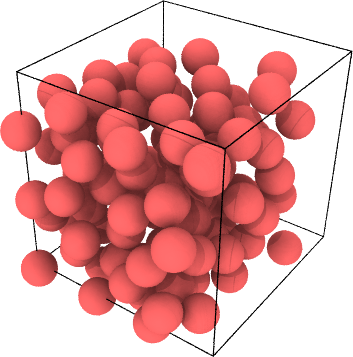
\includegraphics[scale=0.6]{images/example_render}
		\caption{A rendering of one snapshot of the sample simulation produced by Ovito.}
		\label{fig:ovitosample}
	\end{figure}